\chapter{Introduction, Architecture and Infrastructure}

\section{Evolution: From Server Rooms to AI Factories}
\begin{figure}[H]
    \centering
    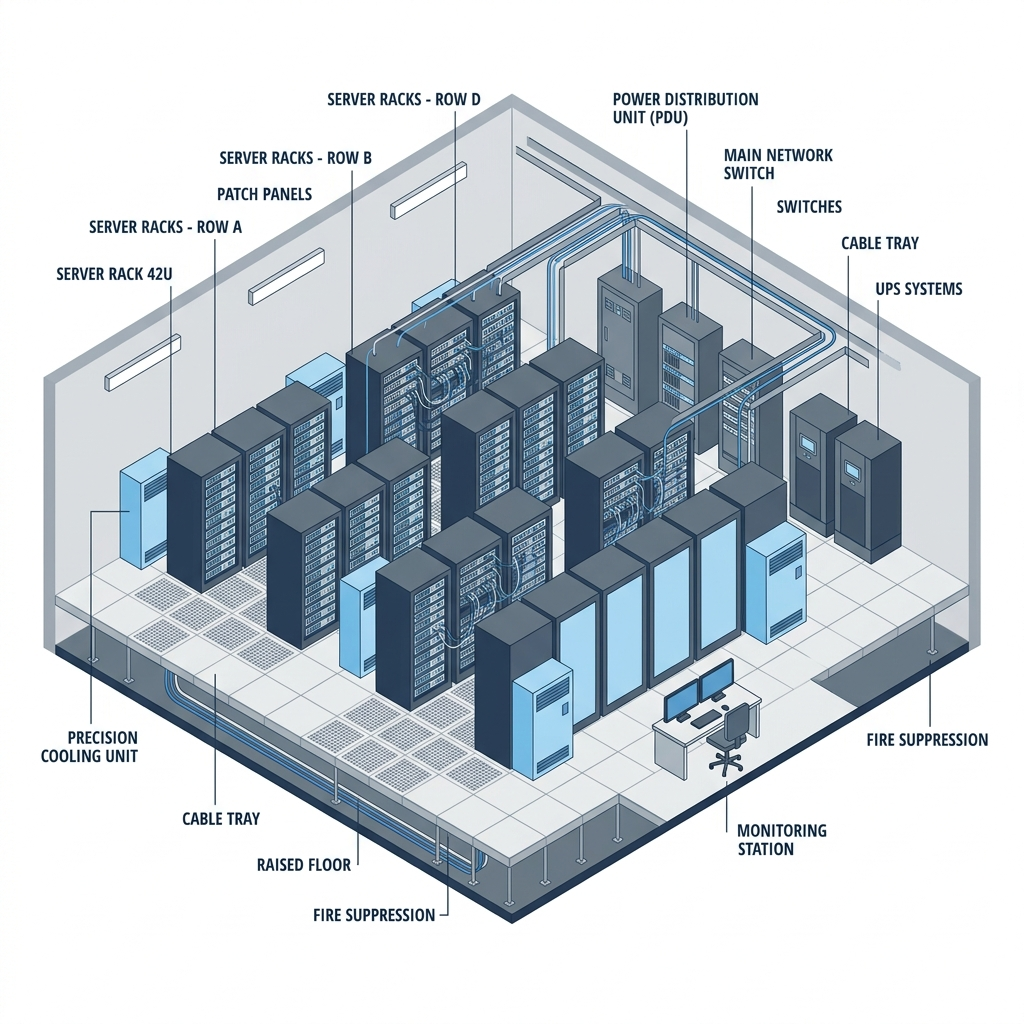
\includegraphics[width=0.8\textwidth]{images/datacenter_isometric.png}
    \caption{Isometric illustration of a modern high-density datacenter.}
\end{figure}
\subsection{From Mainframes to the Dot-Com Bubble}
Historically, centralized computing started in the 60s and 70s with \textbf{Mainframes} (e.g. IBM systems): gigantic cabinets enclosed in sterile rooms ("glass houses") which users accessed via dumb terminals (green screens). In this phase, the system was a monolithic, proprietary, and highly centralized block.
In the 80s and 90s, there was a shift to the \textbf{Client-Server} model, with x86 servers (open architecture) distributed in simple corporate "server rooms", often repurposed closets with a commercial air conditioner and no real engineering design.
At the end of the 90s, the explosion of the Internet led to the \textbf{Dot-Com bubble}: the need to scale globally pushed companies to rent space (Colocation) in gigantic specialized buildings managed by telcos and providers, to ensure 24/7 accessibility. This gave birth to the true modern concept of a Datacenter.

\subsection{The Era of Artificial Intelligence and the Top500}
Today, these are critical infrastructures at a national level, requiring investments of hundreds of millions, if not billions, of euros. 
The explosion of artificial intelligence (AI) has led to the era of \textbf{AI Factories}: industrial complexes capable of absorbing up to 1-2 Gigawatts, the equivalent of an entire city.
The power of these clusters is constantly tracked by two biannual global rankings (started in 1993):
\begin{itemize}
    \item \textbf{Top500:} Measures absolute performance (linear algebra benchmarks in PetaFLOPS).
    \item \textbf{Green500:} Measures energy efficiency (GigaFLOPS per Watt), highlighting the profound \textbf{environmental impact} of these structures.
\end{itemize}

AI has radically altered past paradigms: while traditional Cloud computing uses virtualization to maximize the use of hardware (normally idle for 90\% of the time), AI is the first \textit{workload} that \textbf{fully saturates the physical hardware}. This makes virtualization useless in the AI stack and dictates the use of hardware architectures distributed across tens of thousands of interconnected GPUs.

\section{Fundamentals and Physical Constraints}
The construction of a modern datacenter clashes with engineering limits defined as \textbf{Hard Thresholds}: physical thresholds beyond which it is not simply possible to "scale" (enlarge) a technology, but a radical rethinking becomes necessary.

\begin{warningbox}[Attention: Scale Up vs Scale Out]
\begin{itemize}
    \item \textbf{Scale Out:} adding new nodes or servers to distribute the load.
    \item \textbf{Scale Up:} increasing the capacity of the single node (or, in the electrical case, of the single cable or building).
\end{itemize}
The electrical infrastructure of an entire datacenter is forced to operate in a \textbf{Scale Up} logic: as consumption increases, increasingly thick and expensive copper cables are required.
\end{warningbox}

\subsection{Floating Floor}
\begin{figure}[H]
    \centering
    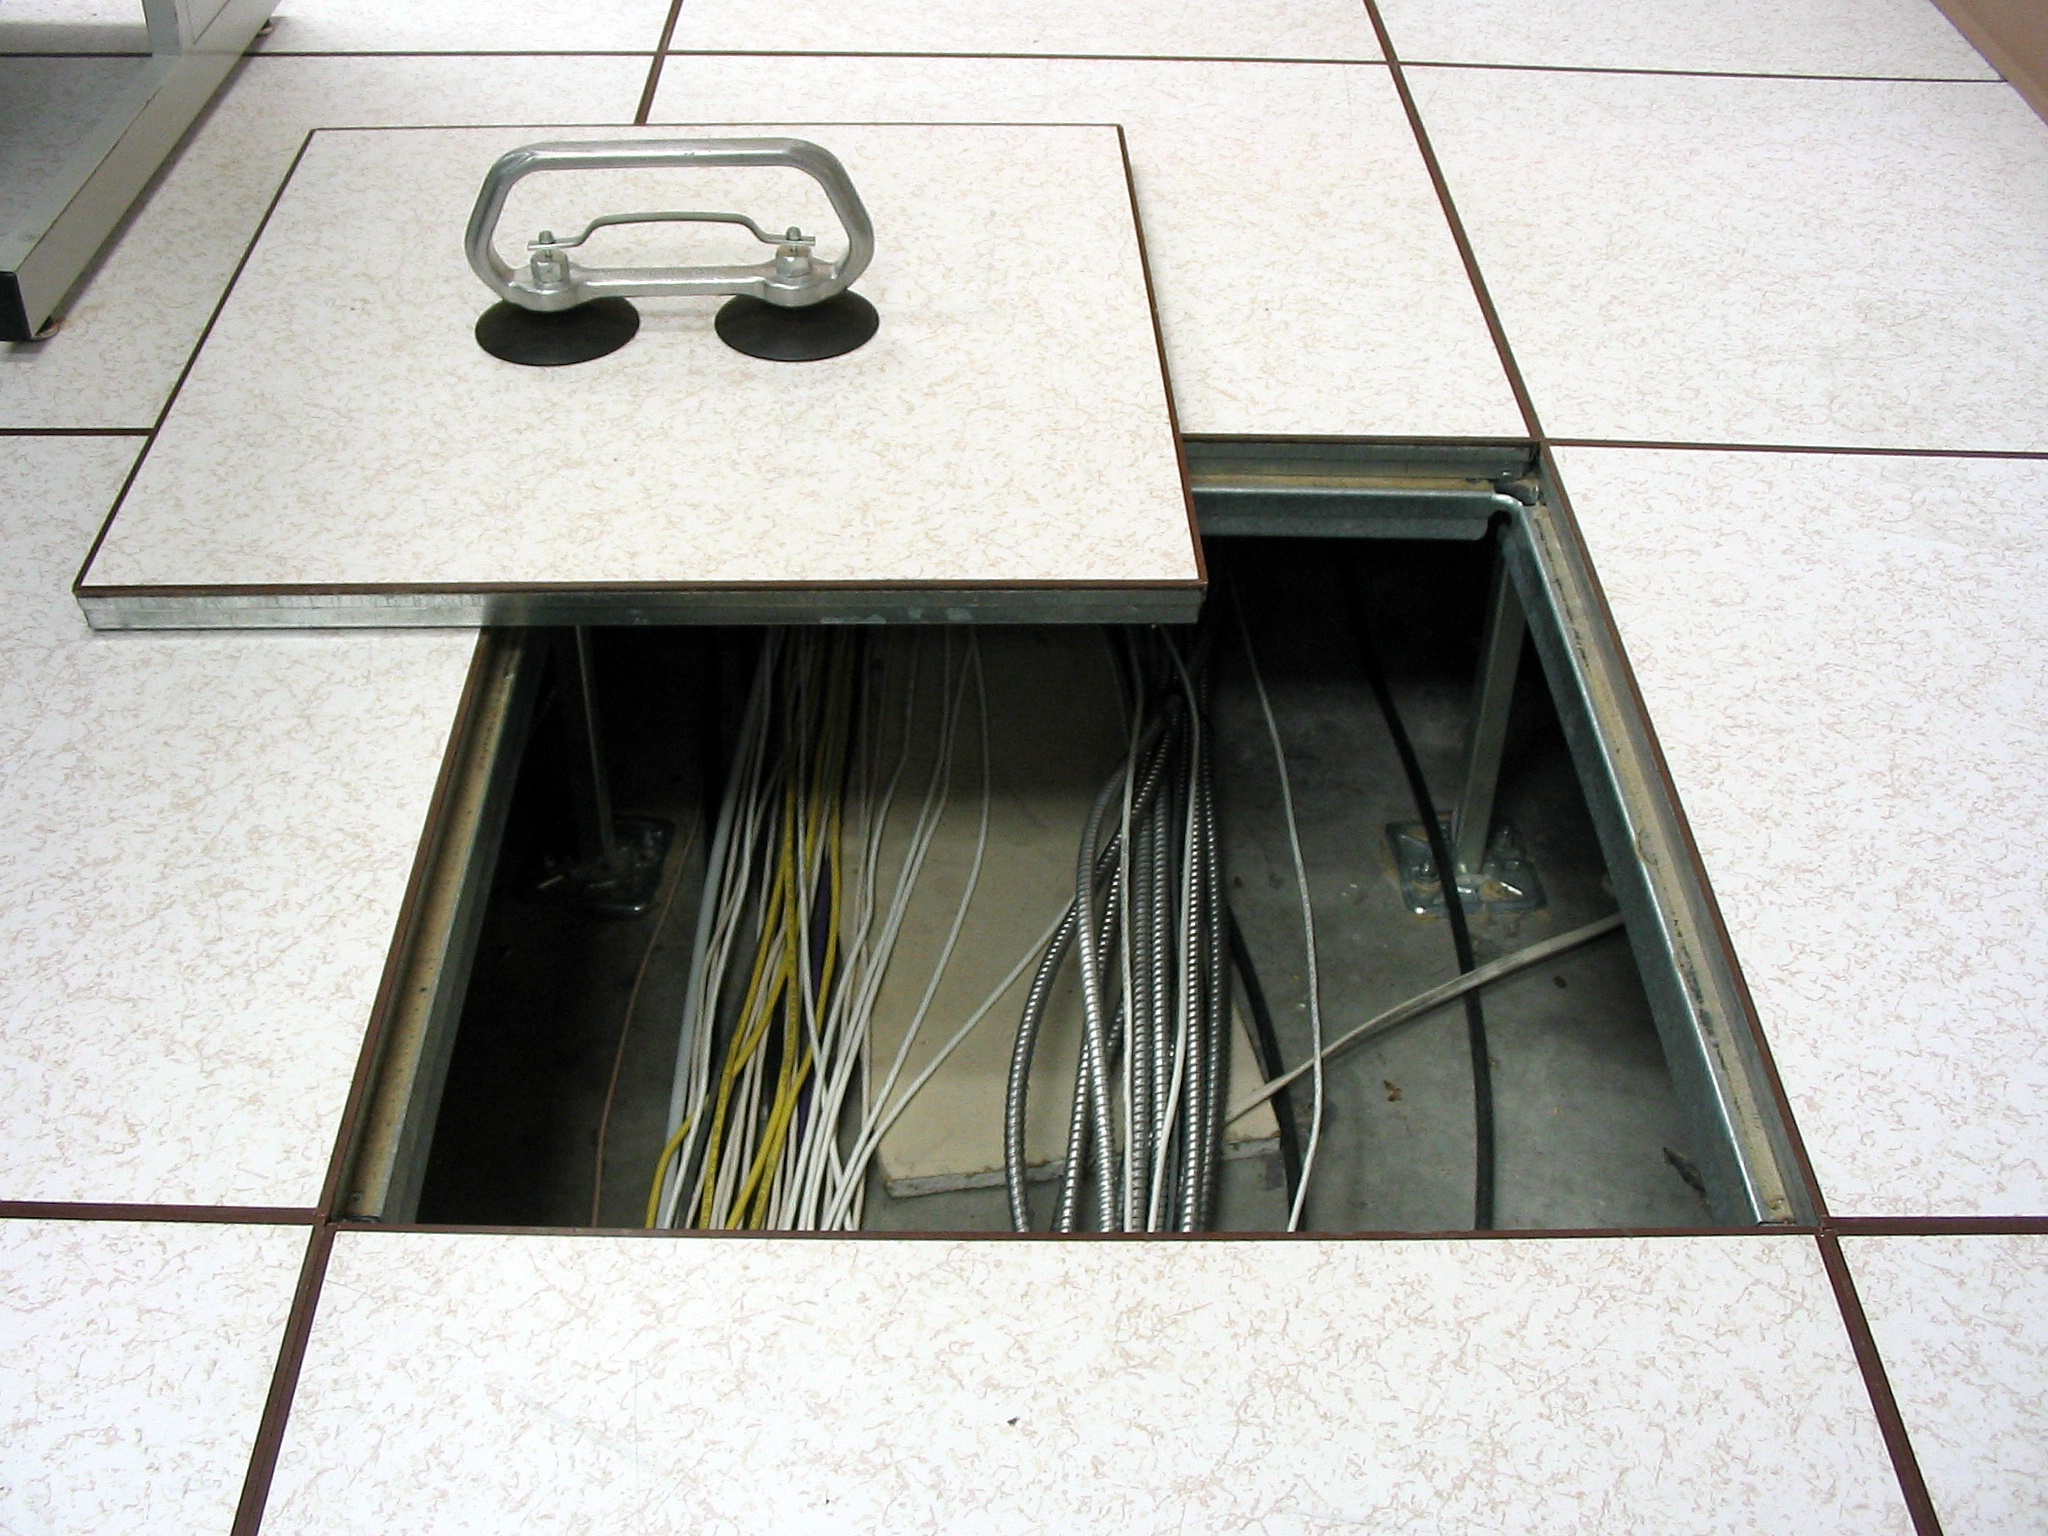
\includegraphics[width=0.7\textwidth]{images/raised_floor.jpg}
    \caption{Lifting of a tile from the raised floor in a data center (Wikimedia Commons).}
\end{figure}
One of the most widespread engineering legacies is the \textbf{Floating Floor} (raised floor). Consisting of panels raised on metal pedestals, in modern DCs it can support up to 1.5 tons per square meter.
The two main advantages are:
\begin{enumerate}
    \item \textbf{Cable management:} orderly routing of cabling infrastructure and plumbing.
    \item \textbf{Air plenum:} creation of a pressurized duct under the floor to distribute cold air from the cooling system towards the grilles positioned in front of the racks.
\end{enumerate}

\section{Cooling and Thermal Management}
Due to the extreme heat density, caused by the high \textbf{TDP (Thermal Design Power)} of new processors (reaching a Kilowatt per single GPU), thermal control has become the most critical aspect of the design. 
Extreme temperatures can melt silicon components; the interruption of the cooling system, combined with the attempt of the server fans to push air, causes exponential thermal increases that can damage the entire room in a few minutes.

\subsection{Air Architecture: CRAC Systems and Flows}
\begin{figure}[H]
    \centering
    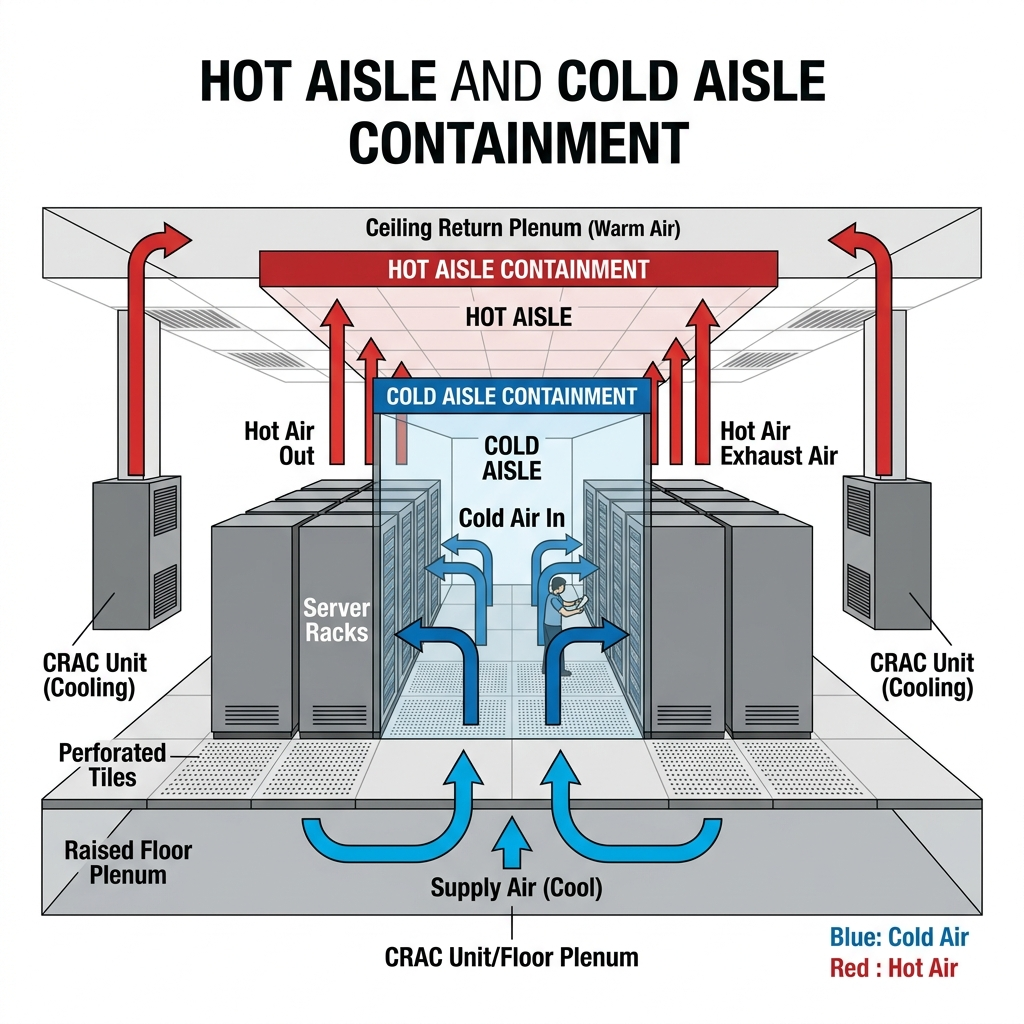
\includegraphics[width=0.8\textwidth]{images/aisle_containment.png}
    \caption{Airflow diagram: Cold Aisle Containment and Hot Aisle.}
\end{figure}
\textbf{CRAC (Computer Room Air Conditioning)} systems rely on the raised floor and the principle of strict separation between the \textit{Cold Aisle} and the \textit{Hot Aisle}. 
The airflow follows a precise path: the CRAC units pump chilled pressurized air into the \textit{plenum} (the space under the raised floor). The air flows out of the perforated grates exactly in front of the racks (Cold Aisle). The server fans suck the air in from the front, cool the internal heatsinks, and expel the blistering hot air out the back into the Hot Aisle, where it rises to the ceiling to return to the CRACs and be cooled again using water heat exchangers (Chillers).

\begin{tipbox}[Golden Rule]
Never mix hot air and cold air. If the flows mix, efficiency plummets and CPUs risk \textit{thermal throttling}. For this reason, glass doors and closed roofs are used to create systems of \textbf{physical containment} for the aisles.
\end{tipbox}

However, air is a terrible thermal conductor. For high loads (Racks beyond 15-20 kW, not to mention modern 200 kW AI racks), CRAC air systems are insufficient.

\subsection{Liquid Cooling}
Liquid cooling is today a de facto standard for high performance computing (HPC):
\begin{itemize}
    \item \textbf{Direct-to-Chip:} water-cooled copper plates placed directly in contact with CPU, GPU and RAM. It removes the need for high-speed fans.
    \item \textbf{Waterless Cooling:} use of dielectric fluids (e.g. glycol) in piping. In case of a spill, they do not cause short circuits.
    \item \textbf{Immersion Cooling:} complete immersion of the motherboard in mineral oil. Eliminates any localized heat point (hot-spot), but makes maintenance complex and expensive.
\end{itemize}

\section{Energy Efficiency (PUE)}
The efficiency of a datacenter is measured with a standard dimensionless value, the \textbf{PUE (Power Usage Effectiveness)}:
\[
PUE = \frac{\text{Total Facility Power}}{\text{IT Equipment Power}}
\]
The closer the PUE is to 1, the higher the efficiency (it means energy is not being wasted on cooling). The best modern data centers have an annual PUE around 1.15 - 1.20.

\begin{warningbox}[The Pitfalls of PUE]
Although PUE is the de facto standard, it presents several critical ambiguities that can be misleading:
\begin{itemize}
    \item \textbf{Impact of Seasonality:} PUE is not a fixed value. A datacenter that exploits outside air cooling (Free Cooling) will measure an excellent PUE (e.g. 1.05) in winter, but will see efficiency plummet (e.g. 1.50) in summer due to the forced activation of mechanical compressors.
    \item \textbf{The Empty Datacenter Paradox:} A newly opened data center with very few servers turned on (very low IT Power) will paradoxically have an abysmal PUE. This is because industrial cooling systems (chillers, pumps) have an unavoidable baseline consumption even when running at minimum, skewing the mathematical fraction.
    \item \textbf{Economic Evaluation (Domestic Splits):} To cool a small server room, installing an industrial plant (PUE 1.3) would cost tens of thousands of euros and require expensive maintenance contracts. Simple "split" domestic air conditioners are often chosen: they bring the PUE to a disastrous 2.0, but they are economically the most sensible choice in terms of initial investment and practical reliability.
\end{itemize}
\end{warningbox}


\section{Security and Continuity}
The logical design follows the so-called \textbf{CIA Triad}:
\begin{itemize}
    \item \textbf{C}onfidentiality
    \item \textbf{I}ntegrity
    \item \textbf{A}vailability
\end{itemize}

Electrical supply is vital. The distribution follows a rigorous chain:
From the external alternating current (AC) grid, it passes to industrial \textbf{UPS (Uninterruptible Power Supply)} (based on huge batteries and pre-compressed spring systems for instantaneous switching) which stabilize the current and prevent micro-interruptions. From the UPS it goes to the hierarchical \textbf{PDU (Power Distribution Unit)}, up to the servers which internally convert AC to direct current (DC).

The need for extreme resilience clashes with practical and geographical limits. The location of data centers must in fact take into account critical variables such as seismic risk, temperature ranges, immediate access to the ultra-high voltage transmission grid and regulatory obligations imposed by GDPR.
